% Options for packages loaded elsewhere
\PassOptionsToPackage{unicode}{hyperref}
\PassOptionsToPackage{hyphens}{url}
%
\documentclass[
]{article}
\usepackage{amsmath,amssymb}
\usepackage{lmodern}
\usepackage{iftex}
\ifPDFTeX
  \usepackage[T1]{fontenc}
  \usepackage[utf8]{inputenc}
  \usepackage{textcomp} % provide euro and other symbols
\else % if luatex or xetex
  \usepackage{unicode-math}
  \defaultfontfeatures{Scale=MatchLowercase}
  \defaultfontfeatures[\rmfamily]{Ligatures=TeX,Scale=1}
\fi
% Use upquote if available, for straight quotes in verbatim environments
\IfFileExists{upquote.sty}{\usepackage{upquote}}{}
\IfFileExists{microtype.sty}{% use microtype if available
  \usepackage[]{microtype}
  \UseMicrotypeSet[protrusion]{basicmath} % disable protrusion for tt fonts
}{}
\makeatletter
\@ifundefined{KOMAClassName}{% if non-KOMA class
  \IfFileExists{parskip.sty}{%
    \usepackage{parskip}
  }{% else
    \setlength{\parindent}{0pt}
    \setlength{\parskip}{6pt plus 2pt minus 1pt}}
}{% if KOMA class
  \KOMAoptions{parskip=half}}
\makeatother
\usepackage{xcolor}
\usepackage[margin=1in]{geometry}
\usepackage{color}
\usepackage{fancyvrb}
\newcommand{\VerbBar}{|}
\newcommand{\VERB}{\Verb[commandchars=\\\{\}]}
\DefineVerbatimEnvironment{Highlighting}{Verbatim}{commandchars=\\\{\}}
% Add ',fontsize=\small' for more characters per line
\usepackage{framed}
\definecolor{shadecolor}{RGB}{248,248,248}
\newenvironment{Shaded}{\begin{snugshade}}{\end{snugshade}}
\newcommand{\AlertTok}[1]{\textcolor[rgb]{0.94,0.16,0.16}{#1}}
\newcommand{\AnnotationTok}[1]{\textcolor[rgb]{0.56,0.35,0.01}{\textbf{\textit{#1}}}}
\newcommand{\AttributeTok}[1]{\textcolor[rgb]{0.77,0.63,0.00}{#1}}
\newcommand{\BaseNTok}[1]{\textcolor[rgb]{0.00,0.00,0.81}{#1}}
\newcommand{\BuiltInTok}[1]{#1}
\newcommand{\CharTok}[1]{\textcolor[rgb]{0.31,0.60,0.02}{#1}}
\newcommand{\CommentTok}[1]{\textcolor[rgb]{0.56,0.35,0.01}{\textit{#1}}}
\newcommand{\CommentVarTok}[1]{\textcolor[rgb]{0.56,0.35,0.01}{\textbf{\textit{#1}}}}
\newcommand{\ConstantTok}[1]{\textcolor[rgb]{0.00,0.00,0.00}{#1}}
\newcommand{\ControlFlowTok}[1]{\textcolor[rgb]{0.13,0.29,0.53}{\textbf{#1}}}
\newcommand{\DataTypeTok}[1]{\textcolor[rgb]{0.13,0.29,0.53}{#1}}
\newcommand{\DecValTok}[1]{\textcolor[rgb]{0.00,0.00,0.81}{#1}}
\newcommand{\DocumentationTok}[1]{\textcolor[rgb]{0.56,0.35,0.01}{\textbf{\textit{#1}}}}
\newcommand{\ErrorTok}[1]{\textcolor[rgb]{0.64,0.00,0.00}{\textbf{#1}}}
\newcommand{\ExtensionTok}[1]{#1}
\newcommand{\FloatTok}[1]{\textcolor[rgb]{0.00,0.00,0.81}{#1}}
\newcommand{\FunctionTok}[1]{\textcolor[rgb]{0.00,0.00,0.00}{#1}}
\newcommand{\ImportTok}[1]{#1}
\newcommand{\InformationTok}[1]{\textcolor[rgb]{0.56,0.35,0.01}{\textbf{\textit{#1}}}}
\newcommand{\KeywordTok}[1]{\textcolor[rgb]{0.13,0.29,0.53}{\textbf{#1}}}
\newcommand{\NormalTok}[1]{#1}
\newcommand{\OperatorTok}[1]{\textcolor[rgb]{0.81,0.36,0.00}{\textbf{#1}}}
\newcommand{\OtherTok}[1]{\textcolor[rgb]{0.56,0.35,0.01}{#1}}
\newcommand{\PreprocessorTok}[1]{\textcolor[rgb]{0.56,0.35,0.01}{\textit{#1}}}
\newcommand{\RegionMarkerTok}[1]{#1}
\newcommand{\SpecialCharTok}[1]{\textcolor[rgb]{0.00,0.00,0.00}{#1}}
\newcommand{\SpecialStringTok}[1]{\textcolor[rgb]{0.31,0.60,0.02}{#1}}
\newcommand{\StringTok}[1]{\textcolor[rgb]{0.31,0.60,0.02}{#1}}
\newcommand{\VariableTok}[1]{\textcolor[rgb]{0.00,0.00,0.00}{#1}}
\newcommand{\VerbatimStringTok}[1]{\textcolor[rgb]{0.31,0.60,0.02}{#1}}
\newcommand{\WarningTok}[1]{\textcolor[rgb]{0.56,0.35,0.01}{\textbf{\textit{#1}}}}
\usepackage{graphicx}
\makeatletter
\def\maxwidth{\ifdim\Gin@nat@width>\linewidth\linewidth\else\Gin@nat@width\fi}
\def\maxheight{\ifdim\Gin@nat@height>\textheight\textheight\else\Gin@nat@height\fi}
\makeatother
% Scale images if necessary, so that they will not overflow the page
% margins by default, and it is still possible to overwrite the defaults
% using explicit options in \includegraphics[width, height, ...]{}
\setkeys{Gin}{width=\maxwidth,height=\maxheight,keepaspectratio}
% Set default figure placement to htbp
\makeatletter
\def\fps@figure{htbp}
\makeatother
\setlength{\emergencystretch}{3em} % prevent overfull lines
\providecommand{\tightlist}{%
  \setlength{\itemsep}{0pt}\setlength{\parskip}{0pt}}
\setcounter{secnumdepth}{-\maxdimen} % remove section numbering
\ifLuaTeX
  \usepackage{selnolig}  % disable illegal ligatures
\fi
\IfFileExists{bookmark.sty}{\usepackage{bookmark}}{\usepackage{hyperref}}
\IfFileExists{xurl.sty}{\usepackage{xurl}}{} % add URL line breaks if available
\urlstyle{same} % disable monospaced font for URLs
\hypersetup{
  pdftitle={Lab Assignment \#4},
  pdfauthor={Nick Noel \& Liz Villa},
  hidelinks,
  pdfcreator={LaTeX via pandoc}}

\title{Lab Assignment \#4}
\author{Nick Noel \& Liz Villa}
\date{Due February 27, 2023}

\begin{document}
\maketitle

\hypertarget{instructions}{%
\section{Instructions}\label{instructions}}

The purpose of this lab is to review simple linear regression and
multiple linear regression strategies from Math 338/439.

In this lab, we will be working with the Boston housing dataset
(\texttt{Boston} in the \texttt{ISLR2} library). This dataset has 506
rows and 13 variables.

\begin{Shaded}
\begin{Highlighting}[]
\FunctionTok{library}\NormalTok{(ISLR2)}
\FunctionTok{library}\NormalTok{(ggplot2)}
\FunctionTok{library}\NormalTok{(dplyr)}
\FunctionTok{library}\NormalTok{(car) }\CommentTok{\# For problem 3}
\FunctionTok{library}\NormalTok{(boot)}
\end{Highlighting}
\end{Shaded}

This lab assignment is worth a total of \textbf{19.5 points}.

\hypertarget{problem-1-bootstrap-estimation-of-standard-error}{%
\section{Problem 1: Bootstrap Estimation of Standard
Error}\label{problem-1-bootstrap-estimation-of-standard-error}}

\hypertarget{part-a-code-0.5-pts}{%
\subsection{Part a (Code: 0.5 pts)}\label{part-a-code-0.5-pts}}

Run the code in the first half of ISLR Lab 5.3.4, ``Estimating the
Accuracy of a Statistic of Interest.'' Put each chunk from the textbook
in its own chunk.

If you are in the actuarial science concentration, you should be
familiar with (or will at some point see) this formula! For the rest of
us, note that \(X\) and \(Y\) are assumed to be the yearly return of two
different financial assets, and \(\alpha\), the quantity to be
estimated, is the fraction of money to be invested in \(X\) such that
the variance (risk) of the total investment
\(\alpha X + (1 - \alpha) Y\) is minimized. In this problem \(\alpha\)
is not the significance level!

\begin{Shaded}
\begin{Highlighting}[]
\NormalTok{alpha.fn }\OtherTok{\textless{}{-}} \ControlFlowTok{function}\NormalTok{(data, index) \{}
\NormalTok{  X }\OtherTok{\textless{}{-}}\NormalTok{ data}\SpecialCharTok{$}\NormalTok{X[index]}
\NormalTok{  Y }\OtherTok{\textless{}{-}}\NormalTok{ data}\SpecialCharTok{$}\NormalTok{Y[index]}
\NormalTok{  (}\FunctionTok{var}\NormalTok{(Y) }\SpecialCharTok{{-}} \FunctionTok{cov}\NormalTok{(X, Y)) }\SpecialCharTok{/}\NormalTok{ (}\FunctionTok{var}\NormalTok{(X) }\SpecialCharTok{+} \FunctionTok{var}\NormalTok{(Y) }\SpecialCharTok{{-}} \DecValTok{2} \SpecialCharTok{*} \FunctionTok{cov}\NormalTok{(X, Y))}
\NormalTok{\}}
\end{Highlighting}
\end{Shaded}

\begin{Shaded}
\begin{Highlighting}[]
\FunctionTok{alpha.fn}\NormalTok{(Portfolio, }\DecValTok{1}\SpecialCharTok{:}\DecValTok{100}\NormalTok{)}
\end{Highlighting}
\end{Shaded}

\begin{verbatim}
## [1] 0.5758321
\end{verbatim}

\begin{Shaded}
\begin{Highlighting}[]
\FunctionTok{set.seed}\NormalTok{(}\DecValTok{7}\NormalTok{)}
\FunctionTok{alpha.fn}\NormalTok{(Portfolio, }\FunctionTok{sample}\NormalTok{(}\DecValTok{100}\NormalTok{, }\DecValTok{100}\NormalTok{, }\AttributeTok{replace =}\NormalTok{ T))}
\end{Highlighting}
\end{Shaded}

\begin{verbatim}
## [1] 0.5385326
\end{verbatim}

\begin{Shaded}
\begin{Highlighting}[]
\FunctionTok{boot}\NormalTok{(Portfolio, alpha.fn, }\AttributeTok{R =} \DecValTok{1000}\NormalTok{)}
\end{Highlighting}
\end{Shaded}

\begin{verbatim}
## 
## ORDINARY NONPARAMETRIC BOOTSTRAP
## 
## 
## Call:
## boot(data = Portfolio, statistic = alpha.fn, R = 1000)
## 
## 
## Bootstrap Statistics :
##      original       bias    std. error
## t1* 0.5758321 0.0007959475  0.08969074
\end{verbatim}

\hypertarget{part-b-code-2-pts}{%
\subsection{Part b (Code: 2 pts)}\label{part-b-code-2-pts}}

According to the instructions for Lab 5.3.4, ``We can implement a
bootstrap analysis by performing this command {[}alpha.fn on a bootstrap
sample{]} many times, recording all of the corresponding estimates for
\(\alpha\), and computing the resulting standard deviation.''

Write a code chunk that performs all of those steps and prints out the
standard deviation. Use 1000 bootstrap samples.

\begin{Shaded}
\begin{Highlighting}[]
\FunctionTok{set.seed}\NormalTok{(}\DecValTok{292}\NormalTok{)}
\NormalTok{bsn }\OtherTok{\textless{}{-}} \DecValTok{1000}
\NormalTok{bsalpha }\OtherTok{\textless{}{-}} \FunctionTok{rep}\NormalTok{(}\ConstantTok{NA}\NormalTok{, bsn)}
\ControlFlowTok{for}\NormalTok{(i }\ControlFlowTok{in} \DecValTok{1}\SpecialCharTok{:}\NormalTok{bsn)\{bsalpha[i] }\OtherTok{=} \FunctionTok{alpha.fn}\NormalTok{(Portfolio, }\FunctionTok{sample}\NormalTok{(}\DecValTok{100}\NormalTok{, }\DecValTok{100}\NormalTok{, }\AttributeTok{replace =}\NormalTok{ T))\}}
\FunctionTok{sd}\NormalTok{(bsalpha)}
\end{Highlighting}
\end{Shaded}

\begin{verbatim}
## [1] 0.08633873
\end{verbatim}

\hypertarget{part-c-code-1-pt}{%
\subsection{Part c (Code: 1 pt)}\label{part-c-code-1-pt}}

Replicate the center panel of textbook Figure 5.10: a histogram of the
bootstrap estimates of \(\alpha\) (from Part b) with a solid pink (or
red) line at the true value of \(\alpha = 0.6\). You may use either base
R plotting commands (which uses \texttt{abline} to add the vertical
line) or the \texttt{ggplot2} package (which adds a \texttt{geom\_vline}
to the plot).

\begin{Shaded}
\begin{Highlighting}[]
\FunctionTok{ggplot}\NormalTok{(}\AttributeTok{mapping =} \FunctionTok{aes}\NormalTok{(bsalpha)) }\SpecialCharTok{+}
  \FunctionTok{geom\_histogram}\NormalTok{(}\AttributeTok{bins =} \DecValTok{12}\NormalTok{, }\AttributeTok{fill =} \StringTok{"steelblue"}\NormalTok{, }\AttributeTok{color =} \StringTok{"black"}\NormalTok{) }\SpecialCharTok{+}
  \FunctionTok{geom\_vline}\NormalTok{(}\AttributeTok{xintercept =} \FloatTok{0.6}\NormalTok{, }\AttributeTok{color =} \StringTok{"pink"}\NormalTok{, }\AttributeTok{size =} \DecValTok{1}\NormalTok{) }\SpecialCharTok{+}
  \FunctionTok{xlab}\NormalTok{(}\StringTok{"alpha"}\NormalTok{)}
\end{Highlighting}
\end{Shaded}

\includegraphics{Lab4_new_files/figure-latex/unnamed-chunk-6-1.pdf}

\hypertarget{part-d-explanation-1-pt}{%
\subsection{Part d (Explanation: 1 pt)}\label{part-d-explanation-1-pt}}

Note that the distribution you graphed in Part c is a sampling
distribution of \(\hat{\alpha}\). Explain why it would be appropriate to
use this sampling distribution to construct a confidence interval for
\(\alpha\), but not to obtain a p-value for a hypothesis test of
\(H_0: \alpha = 0.6\) against \(H_a: \alpha \neq 0.6\).

A confidence interval concerns the estimate of a parameter and
bootstrapping is able to create a distribution which has variability and
distribution similar to the true population. It would not be appropriate
to obtain a p-value for a hypothesis test of \(H_0: \alpha = 0.6\)
against \(H_a: \alpha \neq 0.6\) since we are using simulated values of
alpha rather than true values that accurately reflect the distribution
of the population therefore making the null hypothesis false from the
start.

\hypertarget{problem-2-domain-knowledge-and-exploratory-data-analysis}{%
\section{Problem 2: Domain Knowledge and Exploratory Data
Analysis}\label{problem-2-domain-knowledge-and-exploratory-data-analysis}}

\hypertarget{part-a-explanation-1-pt}{%
\subsection{Part a (Explanation: 1 pt)}\label{part-a-explanation-1-pt}}

Do an Internet search for ``Boston housing dataset'' and answer the
following questions as best you can.

\begin{itemize}
\tightlist
\item
  Who collected this data? How old is this dataset? Answer: Data was
  collected by the U.S. Census Service concerning housing in the area of
  Boston Massachusetts in 1978 (Or around then, 1978 was when the data
  was officially published, possible that the data was collected
  somewhat earlier. )
\item
  What does one row in this dataset represent? Answer: One row in the
  dataset represents a the data collected for a single house on the
  multiple variables.
\end{itemize}

\hypertarget{part-b-explanation-1.5-pts}{%
\subsection{Part b (Explanation: 1.5
pts)}\label{part-b-explanation-1.5-pts}}

In your search, you should eventually come across references to a
\emph{fourteenth} variable, \texttt{B}, which the textbook authors have
removed from the dataset. What does this mysterious variable represent?

Answer: According to a data dictionary we found, B was reported as
follows: ``B - 1000(Bk - 0.63)\^{}2 where Bk is the proportion of blacks
by town''. In simpler terms, the variable B is regarding the proportion
of black people in a town.

Suppose you are a data scientist at Zillow or a similar company whose
housing price models are often used as a reference when people decide
how much to offer to buy or sell a home for. What ethical issues would
arise from using the variable \texttt{B} in your model?

Answer: Using the ethnicity of those around said property as a factor of
the value of the property seems like a very unethical way of determining
the value of a property. The original research was based around the air
pollution of the area so likely dealt with the variable to acknowledge
socioeconomic issues as opposed to putting a value on the property.

\hypertarget{part-c-code-1-pt-explanation-1-pt}{%
\subsection{Part c (Code: 1 pt; Explanation: 1
pt)}\label{part-c-code-1-pt-explanation-1-pt}}

In the next problem we will be trying to predict \texttt{medv} from
\texttt{lstat}. What does the variable \texttt{medv} represent? What are
the measurement units?

Answer: MEDV - Median value of owner-occupied homes in \$1000's

Using the \texttt{ggplot2} package, create a histogram of the variable
\texttt{medv}. Use a \texttt{center} of 35 and a \texttt{binwidth} of 2.

\begin{Shaded}
\begin{Highlighting}[]
\NormalTok{Boston }\SpecialCharTok{\%\textgreater{}\%} 
  \FunctionTok{ggplot}\NormalTok{(}\FunctionTok{aes}\NormalTok{(}\AttributeTok{x =}\NormalTok{ medv)) }\SpecialCharTok{+}
  \FunctionTok{geom\_histogram}\NormalTok{(}\AttributeTok{center =} \DecValTok{35}\NormalTok{, }\AttributeTok{binwidth =} \DecValTok{2}\NormalTok{)}
\end{Highlighting}
\end{Shaded}

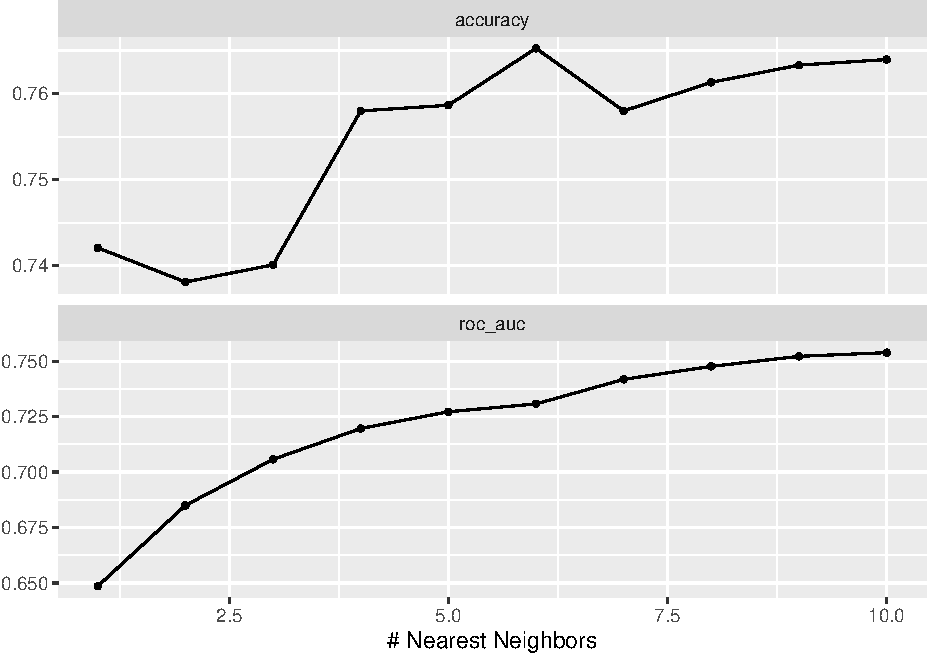
\includegraphics{Lab4_new_files/figure-latex/unnamed-chunk-7-1.pdf}

What looks a bit off about this histogram? Try filling in the
\texttt{filter} function in the chunk below to confirm your suspicions.

\begin{Shaded}
\begin{Highlighting}[]
\NormalTok{Boston }\SpecialCharTok{\%\textgreater{}\%} 
  \FunctionTok{filter}\NormalTok{(medv }\SpecialCharTok{==} \DecValTok{50}\NormalTok{) }\SpecialCharTok{\%\textgreater{}\%}
  \FunctionTok{count}\NormalTok{() }\CommentTok{\# getting sample size without having to summarize}
\end{Highlighting}
\end{Shaded}

The prices were capped at 50,000 and thus any property worth more than
that was lumped into one large group of a value of 50.

\hypertarget{part-d-code-1-pt-explanation-1-pt}{%
\subsection{Part d (Code: 1 pt; Explanation: 1
pt)}\label{part-d-code-1-pt-explanation-1-pt}}

The full documentation for this dataset is somewhat confusing and raises
more questions than answers. For example, \texttt{lstat} is defined as
``\(\frac{1}{2}\) (proportion of adults without some high school
education and proportion of male workers classified as laborers)''
(whatever that means), and \texttt{rad} represents the ``index of
accessibility to radial highways'' as determined by something called the
``MIT Boston Project.''

Other variables are sensibly defined, but are counterintuitive to what
we would expect. Pick either the variable \texttt{age} or \texttt{rm},
and answer the following questions:

\begin{itemize}
\tightlist
\item
  What do you expect this variable would represent, if the observational
  units were houses?
\end{itemize}

Answer: I would expect the variable, age, to represent the age of the
house. * What does this variable actually represent?

Answer: AGE - proportion of owner-occupied units built prior to 1940

\begin{itemize}
\tightlist
\item
  What is the distribution of this variable in the dataset? Include at
  least one graph to support your answer.
\end{itemize}

\begin{Shaded}
\begin{Highlighting}[]
\NormalTok{Boston }\SpecialCharTok{\%\textgreater{}\%} 
  \FunctionTok{ggplot}\NormalTok{(}\FunctionTok{aes}\NormalTok{(}\AttributeTok{x =}\NormalTok{ age)) }\SpecialCharTok{+}
  \FunctionTok{geom\_histogram}\NormalTok{()}
\end{Highlighting}
\end{Shaded}

\begin{verbatim}
## `stat_bin()` using `bins = 30`. Pick better value with `binwidth`.
\end{verbatim}

\includegraphics{Lab4_new_files/figure-latex/unnamed-chunk-8-1.pdf}

\begin{itemize}
\tightlist
\item
  Does this variable appear to have a relationship with the response
  variable \texttt{medv}? Include at least one graph to support your
  answer.
\end{itemize}

\begin{Shaded}
\begin{Highlighting}[]
\NormalTok{Boston }\SpecialCharTok{\%\textgreater{}\%} 
  \FunctionTok{ggplot}\NormalTok{(}\FunctionTok{aes}\NormalTok{(}\AttributeTok{x =}\NormalTok{ age, }\AttributeTok{y =}\NormalTok{ medv)) }\SpecialCharTok{+}
  \FunctionTok{geom\_point}\NormalTok{() }\SpecialCharTok{+}
  \FunctionTok{geom\_smooth}\NormalTok{(}\AttributeTok{method =}\NormalTok{ lm)}
\end{Highlighting}
\end{Shaded}

\begin{verbatim}
## `geom_smooth()` using formula 'y ~ x'
\end{verbatim}

\includegraphics{Lab4_new_files/figure-latex/unnamed-chunk-9-1.pdf}

Based on the above graph there does not seem to be a relationship
between our predictor age, and response, median value of owner-occupied
home.

\hypertarget{problem-3-simple-linear-regression}{%
\section{Problem 3: Simple Linear
Regression}\label{problem-3-simple-linear-regression}}

\hypertarget{part-a-code-0.5-pts-explanation-1-pt}{%
\subsection{Part a (Code: 0.5 pts; Explanation: 1
pt)}\label{part-a-code-0.5-pts-explanation-1-pt}}

Run the code in ISLR Lab 3.6.2. Put each chunk from the textbook in its
own chunk.

\begin{Shaded}
\begin{Highlighting}[]
\FunctionTok{head}\NormalTok{(Boston)}
\end{Highlighting}
\end{Shaded}

\begin{verbatim}
##      crim zn indus chas   nox    rm  age    dis rad tax ptratio lstat medv
## 1 0.00632 18  2.31    0 0.538 6.575 65.2 4.0900   1 296    15.3  4.98 24.0
## 2 0.02731  0  7.07    0 0.469 6.421 78.9 4.9671   2 242    17.8  9.14 21.6
## 3 0.02729  0  7.07    0 0.469 7.185 61.1 4.9671   2 242    17.8  4.03 34.7
## 4 0.03237  0  2.18    0 0.458 6.998 45.8 6.0622   3 222    18.7  2.94 33.4
## 5 0.06905  0  2.18    0 0.458 7.147 54.2 6.0622   3 222    18.7  5.33 36.2
## 6 0.02985  0  2.18    0 0.458 6.430 58.7 6.0622   3 222    18.7  5.21 28.7
\end{verbatim}

\begin{Shaded}
\begin{Highlighting}[]
\NormalTok{lm.fit }\OtherTok{\textless{}{-}} \FunctionTok{lm}\NormalTok{(medv }\SpecialCharTok{\textasciitilde{}}\NormalTok{lstat, }\AttributeTok{data =}\NormalTok{ Boston)}
\end{Highlighting}
\end{Shaded}

\begin{Shaded}
\begin{Highlighting}[]
\NormalTok{lm.fit }\OtherTok{\textless{}{-}} \FunctionTok{lm}\NormalTok{(medv }\SpecialCharTok{\textasciitilde{}}\NormalTok{lstat, }\AttributeTok{data =}\NormalTok{ Boston)}
\CommentTok{\#attach(Boston) I commented this out because I hate using attach but  I understand why we would use it}
\CommentTok{\# lm.fit \textless{}{-} lm(medv ∼ lstat)}
\end{Highlighting}
\end{Shaded}

\begin{Shaded}
\begin{Highlighting}[]
\NormalTok{lm.fit}
\end{Highlighting}
\end{Shaded}

\begin{verbatim}
## 
## Call:
## lm(formula = medv ~ lstat, data = Boston)
## 
## Coefficients:
## (Intercept)        lstat  
##       34.55        -0.95
\end{verbatim}

\begin{Shaded}
\begin{Highlighting}[]
\CommentTok{\# summarise(lm.fit)}
\end{Highlighting}
\end{Shaded}

\begin{Shaded}
\begin{Highlighting}[]
\FunctionTok{names}\NormalTok{(lm.fit)}
\end{Highlighting}
\end{Shaded}

\begin{verbatim}
##  [1] "coefficients"  "residuals"     "effects"       "rank"         
##  [5] "fitted.values" "assign"        "qr"            "df.residual"  
##  [9] "xlevels"       "call"          "terms"         "model"
\end{verbatim}

\begin{Shaded}
\begin{Highlighting}[]
\FunctionTok{coef}\NormalTok{(lm.fit)}
\end{Highlighting}
\end{Shaded}

\begin{verbatim}
## (Intercept)       lstat 
##  34.5538409  -0.9500494
\end{verbatim}

\begin{Shaded}
\begin{Highlighting}[]
\FunctionTok{confint}\NormalTok{(lm.fit)}
\end{Highlighting}
\end{Shaded}

\begin{verbatim}
##                 2.5 %     97.5 %
## (Intercept) 33.448457 35.6592247
## lstat       -1.026148 -0.8739505
\end{verbatim}

\begin{Shaded}
\begin{Highlighting}[]
\FunctionTok{predict}\NormalTok{(lm.fit, }\FunctionTok{data.frame}\NormalTok{(}\AttributeTok{lstat =}\NormalTok{ (}\FunctionTok{c}\NormalTok{(}\DecValTok{5}\NormalTok{, }\DecValTok{10}\NormalTok{, }\DecValTok{15}\NormalTok{))),}\AttributeTok{interval =} \StringTok{"confidence"}\NormalTok{)}
\end{Highlighting}
\end{Shaded}

\begin{verbatim}
##        fit      lwr      upr
## 1 29.80359 29.00741 30.59978
## 2 25.05335 24.47413 25.63256
## 3 20.30310 19.73159 20.87461
\end{verbatim}

\begin{Shaded}
\begin{Highlighting}[]
\FunctionTok{predict}\NormalTok{(lm.fit, }\FunctionTok{data.frame}\NormalTok{(}\AttributeTok{lstat =}\NormalTok{ (}\FunctionTok{c}\NormalTok{(}\DecValTok{5}\NormalTok{, }\DecValTok{10}\NormalTok{, }\DecValTok{15}\NormalTok{))),}\AttributeTok{interval =} \StringTok{"prediction"}\NormalTok{)}
\end{Highlighting}
\end{Shaded}

\begin{verbatim}
##        fit       lwr      upr
## 1 29.80359 17.565675 42.04151
## 2 25.05335 12.827626 37.27907
## 3 20.30310  8.077742 32.52846
\end{verbatim}

\begin{Shaded}
\begin{Highlighting}[]
\FunctionTok{plot}\NormalTok{(Boston}\SpecialCharTok{$}\NormalTok{lstat, Boston}\SpecialCharTok{$}\NormalTok{medv)}
\FunctionTok{abline}\NormalTok{(lm.fit)}
\end{Highlighting}
\end{Shaded}

\includegraphics{Lab4_new_files/figure-latex/unnamed-chunk-17-1.pdf}

\begin{Shaded}
\begin{Highlighting}[]
\FunctionTok{plot}\NormalTok{(Boston}\SpecialCharTok{$}\NormalTok{lstat,Boston}\SpecialCharTok{$}\NormalTok{medv)}
\FunctionTok{abline}\NormalTok{(lm.fit, }\AttributeTok{lwd =} \DecValTok{3}\NormalTok{)}
\FunctionTok{abline}\NormalTok{(lm.fit, }\AttributeTok{lwd =} \DecValTok{3}\NormalTok{, }\AttributeTok{col =} \StringTok{" red "}\NormalTok{)}
\end{Highlighting}
\end{Shaded}

\includegraphics{Lab4_new_files/figure-latex/unnamed-chunk-18-1.pdf}

\begin{Shaded}
\begin{Highlighting}[]
\FunctionTok{plot}\NormalTok{(Boston}\SpecialCharTok{$}\NormalTok{lstat, Boston}\SpecialCharTok{$}\NormalTok{medv, }\AttributeTok{col =} \StringTok{" red "}\NormalTok{)}
\end{Highlighting}
\end{Shaded}

\includegraphics{Lab4_new_files/figure-latex/unnamed-chunk-18-2.pdf}

\begin{Shaded}
\begin{Highlighting}[]
\FunctionTok{plot}\NormalTok{(Boston}\SpecialCharTok{$}\NormalTok{lstat, Boston}\SpecialCharTok{$}\NormalTok{medv, }\AttributeTok{pch =} \DecValTok{20}\NormalTok{) }
\end{Highlighting}
\end{Shaded}

\includegraphics{Lab4_new_files/figure-latex/unnamed-chunk-18-3.pdf}

\begin{Shaded}
\begin{Highlighting}[]
\FunctionTok{plot}\NormalTok{(Boston}\SpecialCharTok{$}\NormalTok{lstat, Boston}\SpecialCharTok{$}\NormalTok{medv, }\AttributeTok{pch =} \StringTok{"+"}\NormalTok{)}
\end{Highlighting}
\end{Shaded}

\includegraphics{Lab4_new_files/figure-latex/unnamed-chunk-18-4.pdf}

\begin{Shaded}
\begin{Highlighting}[]
\FunctionTok{plot}\NormalTok{(}\DecValTok{1}\SpecialCharTok{:}\DecValTok{20}\NormalTok{, }\DecValTok{1}\SpecialCharTok{:}\DecValTok{20}\NormalTok{, }\AttributeTok{pch =} \DecValTok{1}\SpecialCharTok{:}\DecValTok{20}\NormalTok{)}
\end{Highlighting}
\end{Shaded}

\includegraphics{Lab4_new_files/figure-latex/unnamed-chunk-18-5.pdf}

\begin{Shaded}
\begin{Highlighting}[]
\FunctionTok{par}\NormalTok{(}\AttributeTok{mfrow =} \FunctionTok{c}\NormalTok{(}\DecValTok{2}\NormalTok{, }\DecValTok{2}\NormalTok{))}
\FunctionTok{plot}\NormalTok{(lm.fit)}
\end{Highlighting}
\end{Shaded}

\includegraphics{Lab4_new_files/figure-latex/unnamed-chunk-19-1.pdf}

\begin{Shaded}
\begin{Highlighting}[]
\FunctionTok{plot}\NormalTok{(}\FunctionTok{predict}\NormalTok{(lm.fit), }\FunctionTok{residuals}\NormalTok{(lm.fit))}
\end{Highlighting}
\end{Shaded}

\includegraphics{Lab4_new_files/figure-latex/unnamed-chunk-20-1.pdf}

\begin{Shaded}
\begin{Highlighting}[]
\FunctionTok{plot}\NormalTok{(}\FunctionTok{predict}\NormalTok{(lm.fit), }\FunctionTok{rstudent}\NormalTok{(lm.fit))}
\end{Highlighting}
\end{Shaded}

\includegraphics{Lab4_new_files/figure-latex/unnamed-chunk-20-2.pdf}

\begin{Shaded}
\begin{Highlighting}[]
\FunctionTok{plot}\NormalTok{(}\FunctionTok{hatvalues}\NormalTok{(lm.fit))}
\end{Highlighting}
\end{Shaded}

\includegraphics{Lab4_new_files/figure-latex/unnamed-chunk-21-1.pdf}

\begin{Shaded}
\begin{Highlighting}[]
\FunctionTok{which.max}\NormalTok{(}\FunctionTok{hatvalues}\NormalTok{(lm.fit))}
\end{Highlighting}
\end{Shaded}

\begin{verbatim}
## 375 
## 375
\end{verbatim}

Briefly explain what the \texttt{confint()} and \texttt{predict()}
functions output when applied to a linear model.

Answer: ``confint()'' produces a confidence interval for the coefficient
estimates, since these are not known values we estimate them and
confint() just allows us to see the spread of possible values.
``predict()'' on the other hand produces a confidence interval or
prediction interval for the prediction of y based on whatever the x
variable may be.

\hypertarget{part-b-explanation-2.5-pts}{%
\subsection{Part b (Explanation: 2.5
pts)}\label{part-b-explanation-2.5-pts}}

Write out the equation of the least-squares line relating \texttt{lstat}
and \texttt{medv}. Write two sentences interpreting the parameter
estimates (one for slope, one for intercept) in the context of the data.
Remember to use the right observational units!

medv = 34.55 - 0.95(lstat) + \(\epsilon\)

The parameters of this equation is estimating the median value of the
owners home in 1000s and our model has estimated that when ``\% lower
status of the population'' or in context of the data, ``proportion of
adults without some high school education and proportion of male workers
classified as laborers'' is equal to 0 the value is equal to 34,550
dollars. Our variable, ``lstat'', which again is ``\% lower status of
the population'', for every percentage increase of this value we would
expect to see a decrease in the value of the property of approximately
950 dollars.

Given the issue raised in Problem 1d with the \texttt{lstat}
interpretation, let's just say in our interpretations that
\texttt{lstat} represents the percentage of people in the neighborhood
considered lower class.

Answer: This would then be an incorrect interpretation of the model as
this would change the interpretation of our model to be based on class
of citizens and not the proportion of adults without some high school
education and proportion of male workers classified as laborers

\hypertarget{part-c-explanation-1.5-pts}{%
\subsection{Part c (Explanation: 1.5
pts)}\label{part-c-explanation-1.5-pts}}

\begin{Shaded}
\begin{Highlighting}[]
\FunctionTok{par}\NormalTok{(}\AttributeTok{mfrow =} \FunctionTok{c}\NormalTok{(}\DecValTok{2}\NormalTok{, }\DecValTok{2}\NormalTok{))}
\FunctionTok{plot}\NormalTok{(lm.fit)}
\end{Highlighting}
\end{Shaded}

\includegraphics{Lab4_new_files/figure-latex/unnamed-chunk-22-1.pdf}

Refer to the diagnostic plots you created in Part (a) to answer the
following questions:

\begin{itemize}
\tightlist
\item
  Why do the lab instructions claim that ``there is some evidence of
  non-linearity''?
\end{itemize}

Answer: Based on the Residuals versus Leverage as well as the residuals
versus fitted we see the potential evidence of non-linearity in favor of
a skewed right model.

\begin{itemize}
\tightlist
\item
  Do you believe that the residuals are normally distributed? Why or why
  not?
\end{itemize}

Answer:Based on our QQ plot our residuals are not likely normally
distributed but instead skewed right.

\begin{itemize}
\tightlist
\item
  Do you believe that the response variable is homoskedastic (the
  residuals have roughly constant variance across the entire predictor
  range)? Why or why not?
\end{itemize}

Answer: I do not believe the response variable to be homoskedastic since
there seems to be a downward trend in the data regarding residuals
versus predicted values.

\hypertarget{problem-4-multiple-linear-regression}{%
\section{Problem 4: Multiple Linear
Regression}\label{problem-4-multiple-linear-regression}}

\hypertarget{part-a-code-0.5-pts-explanation-1-pt-1}{%
\subsection{Part a (Code: 0.5 pts; Explanation: 1
pt)}\label{part-a-code-0.5-pts-explanation-1-pt-1}}

Run the code in ISLR Lab 3.6.3. Put each chunk from the textbook in its
own chunk. (Note that you will have to install the \texttt{car}
package.)

\begin{Shaded}
\begin{Highlighting}[]
\NormalTok{lm.fit }\OtherTok{\textless{}{-}} \FunctionTok{lm}\NormalTok{(}\AttributeTok{data =}\NormalTok{ Boston, medv }\SpecialCharTok{\textasciitilde{}}\NormalTok{ lstat }\SpecialCharTok{+}\NormalTok{ age)}
\FunctionTok{summary}\NormalTok{(lm.fit)}
\end{Highlighting}
\end{Shaded}

\begin{verbatim}
## 
## Call:
## lm(formula = medv ~ lstat + age, data = Boston)
## 
## Residuals:
##     Min      1Q  Median      3Q     Max 
## -15.981  -3.978  -1.283   1.968  23.158 
## 
## Coefficients:
##             Estimate Std. Error t value Pr(>|t|)    
## (Intercept) 33.22276    0.73085  45.458  < 2e-16 ***
## lstat       -1.03207    0.04819 -21.416  < 2e-16 ***
## age          0.03454    0.01223   2.826  0.00491 ** 
## ---
## Signif. codes:  0 '***' 0.001 '**' 0.01 '*' 0.05 '.' 0.1 ' ' 1
## 
## Residual standard error: 6.173 on 503 degrees of freedom
## Multiple R-squared:  0.5513, Adjusted R-squared:  0.5495 
## F-statistic:   309 on 2 and 503 DF,  p-value: < 2.2e-16
\end{verbatim}

\begin{Shaded}
\begin{Highlighting}[]
\NormalTok{lm.fit }\OtherTok{\textless{}{-}} \FunctionTok{lm}\NormalTok{(}\AttributeTok{data =}\NormalTok{ Boston, medv }\SpecialCharTok{\textasciitilde{}}\NormalTok{ .)}
\FunctionTok{summary}\NormalTok{(lm.fit)}
\end{Highlighting}
\end{Shaded}

\begin{verbatim}
## 
## Call:
## lm(formula = medv ~ ., data = Boston)
## 
## Residuals:
##      Min       1Q   Median       3Q      Max 
## -15.1304  -2.7673  -0.5814   1.9414  26.2526 
## 
## Coefficients:
##               Estimate Std. Error t value Pr(>|t|)    
## (Intercept)  41.617270   4.936039   8.431 3.79e-16 ***
## crim         -0.121389   0.033000  -3.678 0.000261 ***
## zn            0.046963   0.013879   3.384 0.000772 ***
## indus         0.013468   0.062145   0.217 0.828520    
## chas          2.839993   0.870007   3.264 0.001173 ** 
## nox         -18.758022   3.851355  -4.870 1.50e-06 ***
## rm            3.658119   0.420246   8.705  < 2e-16 ***
## age           0.003611   0.013329   0.271 0.786595    
## dis          -1.490754   0.201623  -7.394 6.17e-13 ***
## rad           0.289405   0.066908   4.325 1.84e-05 ***
## tax          -0.012682   0.003801  -3.337 0.000912 ***
## ptratio      -0.937533   0.132206  -7.091 4.63e-12 ***
## lstat        -0.552019   0.050659 -10.897  < 2e-16 ***
## ---
## Signif. codes:  0 '***' 0.001 '**' 0.01 '*' 0.05 '.' 0.1 ' ' 1
## 
## Residual standard error: 4.798 on 493 degrees of freedom
## Multiple R-squared:  0.7343, Adjusted R-squared:  0.7278 
## F-statistic: 113.5 on 12 and 493 DF,  p-value: < 2.2e-16
\end{verbatim}

\begin{Shaded}
\begin{Highlighting}[]
\FunctionTok{library}\NormalTok{(car)}
\FunctionTok{vif}\NormalTok{(lm.fit)}
\end{Highlighting}
\end{Shaded}

\begin{verbatim}
##     crim       zn    indus     chas      nox       rm      age      dis 
## 1.767486 2.298459 3.987181 1.071168 4.369093 1.912532 3.088232 3.954037 
##      rad      tax  ptratio    lstat 
## 7.445301 9.002158 1.797060 2.870777
\end{verbatim}

\begin{Shaded}
\begin{Highlighting}[]
\NormalTok{lm.fit1 }\OtherTok{\textless{}{-}} \FunctionTok{lm}\NormalTok{(}\AttributeTok{data =}\NormalTok{ Boston, medv }\SpecialCharTok{\textasciitilde{}}\NormalTok{ . }\SpecialCharTok{{-}}\NormalTok{age)}
\FunctionTok{summary}\NormalTok{(lm.fit1)}
\end{Highlighting}
\end{Shaded}

\begin{verbatim}
## 
## Call:
## lm(formula = medv ~ . - age, data = Boston)
## 
## Residuals:
##      Min       1Q   Median       3Q      Max 
## -15.1851  -2.7330  -0.6116   1.8555  26.3838 
## 
## Coefficients:
##               Estimate Std. Error t value Pr(>|t|)    
## (Intercept)  41.525128   4.919684   8.441 3.52e-16 ***
## crim         -0.121426   0.032969  -3.683 0.000256 ***
## zn            0.046512   0.013766   3.379 0.000785 ***
## indus         0.013451   0.062086   0.217 0.828577    
## chas          2.852773   0.867912   3.287 0.001085 ** 
## nox         -18.485070   3.713714  -4.978 8.91e-07 ***
## rm            3.681070   0.411230   8.951  < 2e-16 ***
## dis          -1.506777   0.192570  -7.825 3.12e-14 ***
## rad           0.287940   0.066627   4.322 1.87e-05 ***
## tax          -0.012653   0.003796  -3.333 0.000923 ***
## ptratio      -0.934649   0.131653  -7.099 4.39e-12 ***
## lstat        -0.547409   0.047669 -11.483  < 2e-16 ***
## ---
## Signif. codes:  0 '***' 0.001 '**' 0.01 '*' 0.05 '.' 0.1 ' ' 1
## 
## Residual standard error: 4.794 on 494 degrees of freedom
## Multiple R-squared:  0.7343, Adjusted R-squared:  0.7284 
## F-statistic: 124.1 on 11 and 494 DF,  p-value: < 2.2e-16
\end{verbatim}

\begin{Shaded}
\begin{Highlighting}[]
\NormalTok{lm.fit1 }\OtherTok{\textless{}{-}} \FunctionTok{update}\NormalTok{(lm.fit,}\SpecialCharTok{\textasciitilde{}}\NormalTok{.}\SpecialCharTok{{-}}\NormalTok{age)}
\end{Highlighting}
\end{Shaded}

Briefly explain what the \texttt{vif()} and \texttt{update()} functions
do when applied to a linear model.

``vif()'' can be used to compute variance inflation factors. the
update() function when applied to a linear model updates our model by
changing the predictors of the model, in our case it what to keep all
others and remove the age variable.

\hypertarget{part-b-code-0.5-pts-explanation-1-pt}{%
\subsection{Part b (Code: 0.5 pts; Explanation: 1
pt)}\label{part-b-code-0.5-pts-explanation-1-pt}}

Jumping straight into modeling without looking at the data is a very bad
idea. Create a scatterplot matrix showing only the three variables in
the first \texttt{lm.fit} object (\texttt{medv}, \texttt{lstat},
\texttt{age}).

\begin{Shaded}
\begin{Highlighting}[]
\NormalTok{lm.fit }\OtherTok{\textless{}{-}} \FunctionTok{lm}\NormalTok{(}\AttributeTok{data =}\NormalTok{ Boston, medv }\SpecialCharTok{\textasciitilde{}}\NormalTok{ lstat }\SpecialCharTok{+}\NormalTok{ age)}
\FunctionTok{scatterplotMatrix}\NormalTok{(}\SpecialCharTok{\textasciitilde{}}\NormalTok{ medv}\SpecialCharTok{+}\NormalTok{lstat }\SpecialCharTok{+}\NormalTok{ age, }\AttributeTok{data =}\NormalTok{ Boston)}
\end{Highlighting}
\end{Shaded}

\includegraphics{Lab4_new_files/figure-latex/unnamed-chunk-28-1.pdf}

\begin{Shaded}
\begin{Highlighting}[]
\FunctionTok{cor}\NormalTok{(Boston }\SpecialCharTok{\%\textgreater{}\%} \FunctionTok{select}\NormalTok{(lstat,age))}
\end{Highlighting}
\end{Shaded}

\begin{verbatim}
##           lstat       age
## lstat 1.0000000 0.6023385
## age   0.6023385 1.0000000
\end{verbatim}

Do you see any evidence of nonlinearity? Any evidence of collinearity?
Explain your reasoning.

Answer: In the plots of both our x variables, lstat and age, against
medv we see clear trends which inclines us to say the relationship
between our prediction and response variables are not linear. There may
be some signs of colinearity as well, as the relationship between our
variables lstat and age have a correlation value of .6 so it is not too
bad.

\end{document}
